\section{What is Upkeeper.}\label{index_whatis}
Upkeeper is a process control, monitor, with auditing system.

Upkeeper consists of 4 logical components
\begin{DoxyItemize}
\item Buddy -\/ The individual process monitor.
\item Controller -\/ The audit and control service.
\item Libupkeeper -\/ The client library.
\item Clients -\/ tools and utilities to interact with upkeeper.
\end{DoxyItemize}

upkeeper's is almost between DJB's daemontools, and freedesktop's systemd, in terms of functionality and capabilities. However, it adds the additional capability of recording state changes of monitored processes to a data store, which can then be interogated, preferably via the API, for the purpose troubleshooting, event correlation, metrics collection, trending, and analysis.\section{How the system works:}\label{index_howitworks}
A high-\/level view of the interaction between components is as follows:

\begin{center}

\begin{DoxyImageNoCaption}
  \mbox{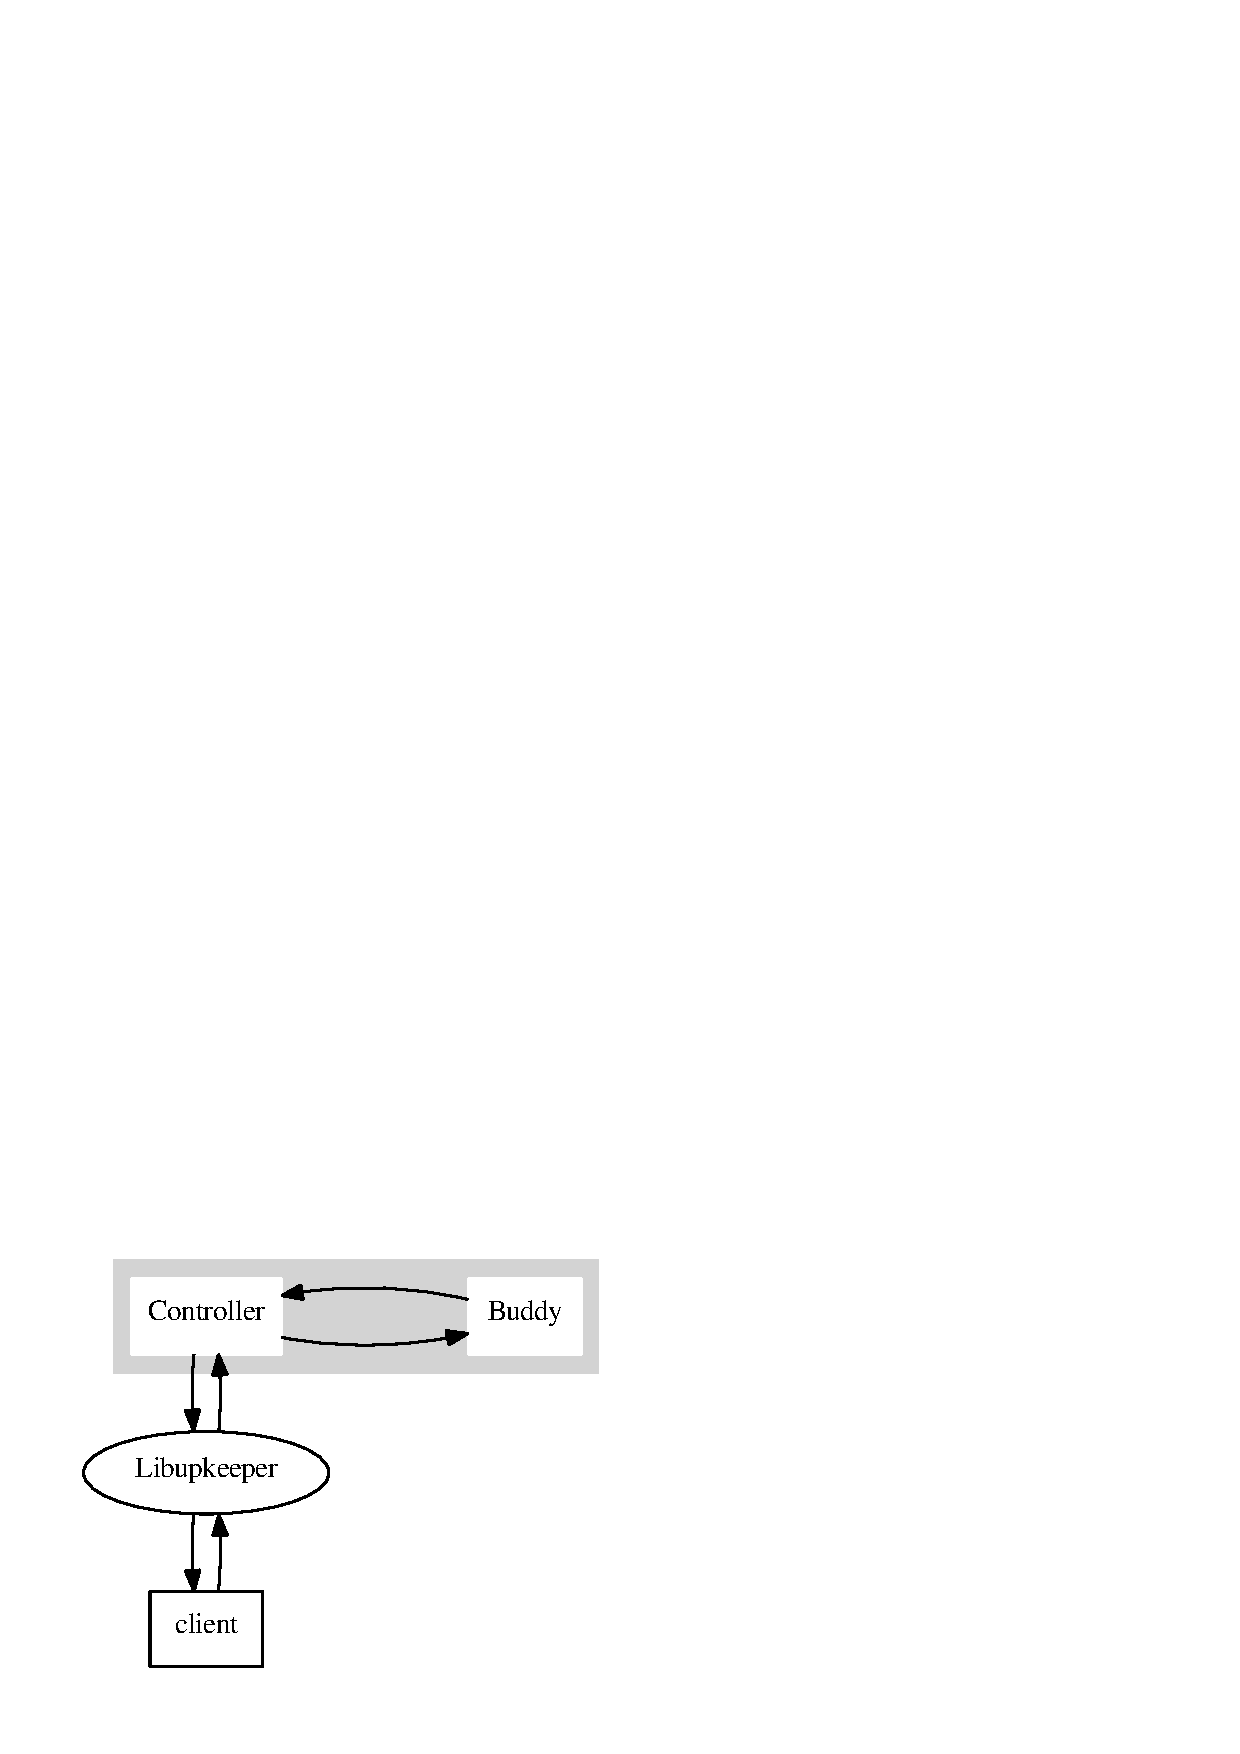
\includegraphics[width=\textwidth]{dot_inline_dotgraph_1}}
\end{DoxyImageNoCaption}
\end{center}


Controller is responsible for maintaining the configuration of buddy process, establishing the environment in which buddy runs, and invoking buddies. Once a buddy has been invoked, it runs autonymously until terminated. Excessive care has been taken to ensure that a buddy will not terminate under normal, and even some rather extraordinary, circumstances.

Buddy is a simplistic-\/by-\/design component that primarily just sits in a loop and waits for the process its monitoring to change terminate, or otherwise catch a signal. To communicate status changes with controller, buddy listens to a socket, which controller polls at a configurable interval. If controller dies for some reason, buddy has a user-\/configurably sized ringbuffer which will backlog status events, and report them once a controller becomes available. If a ringbuffer becomes $>$= 75\% full, or if a buddy is attempting to terminate while having events in its ringbuffer, the buddy will attempt to contact a controller on the controller's domain socket, as a last-\/resort.

The environment buddy runs in is a directory structure with files and symlinks that buddy uses to invoke actions, and log output. \begin{center}

\begin{DoxyImageNoCaption}
  \mbox{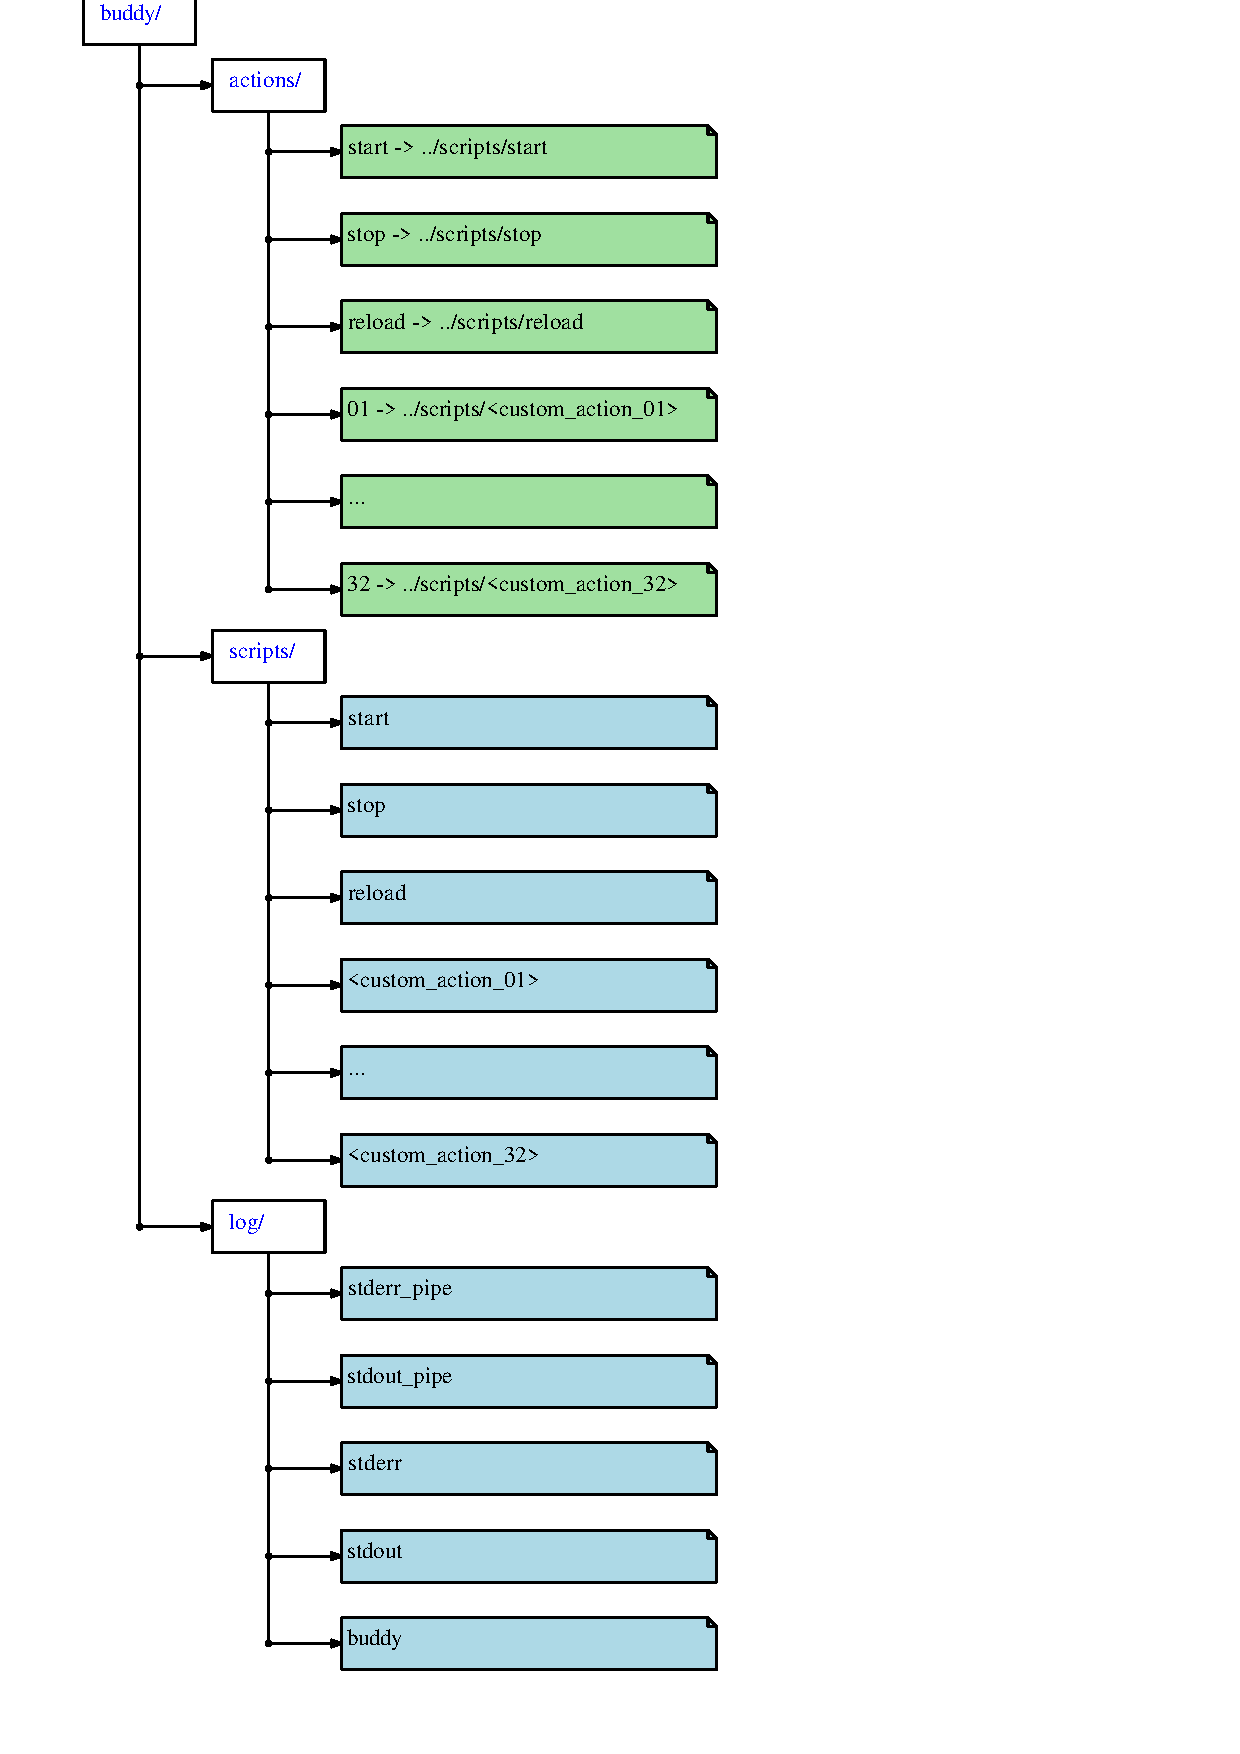
\includegraphics[width=\textwidth]{dot_inline_dotgraph_2}}
\end{DoxyImageNoCaption}
\end{center}


Clients consist of things like \char`\"{}uptop\char`\"{}, which is a status reporting tool that is similar to the common \char`\"{}top\char`\"{} utility. Clients communicate with controller via the API provided in libupkeeper. Hence, you can easily create any client you require, including metrics reporting and/or monitoring and alerting systems.

To explain this, the following sequence chart demonstrates how the components interact:

Start a managed process:

\begin{center}

\begin{DoxyImageNoCaption}  \mbox{\includegraphics{inline_mscgraph_1}}
\end{DoxyImageNoCaption}
\end{center}


Whereas a read-\/only process, such as subscribing to, and receiving events over time would look like this:

\begin{center}

\begin{DoxyImageNoCaption}  \mbox{\includegraphics{inline_mscgraph_2}}
\end{DoxyImageNoCaption}
\end{center}
\section{Sample Configuration.}\label{index_sampleconfig}
\begin{DoxyVerb}
{
    // StateDir
    // Path to variable state-dir for controller and buddies
    "StateDir": "/usr/var/upkeeper",

    // SvcConfigPath
    // Path to location of service configuration files
    "SvcConfigPath": "/usr/etc/upkeeper.d",

    // SvcRunPath
    // Path to location to setup and run buddies
    "SvcRunPath": "/usr/var/upkeeper/buddies",

    // Path to the buddy executable
    "UpkBuddyPath": "/usr/libexec/upk_buddy",

    // How frequently buddy sockets should be polled for events
    // in seconds and fractions of a second
    "BuddyPollingInterval": 0.5,

    // ServiceDefaults:
    "ServiceDefaults": {
        "Provides": Null,
        "UUID": Null,
        "ShortDescription": Null,
        "LongDescription": Null,
        "Prerequisites": Null,
        "StartPriority": 0,
        "BuddyShutdownTimeout": -1,
        "KillTimeout": 60,
        "UserMaxRestarts": Null,
        "UserRestartWindow": Null,
        "UserRateLimit": Null,
        "RandomizeRateLimit": false,
        "SetUID": 0,
        "SetGID": 0,
        "RingbufferSize": 64,
        "ReconnectRetries": 10,
        "ExecStart": Null,
        "StartScript": "#!/bin/sh\nexec %(EXEC_START)\n",
        "ExecStop": "kill",
        "StopScript": "#!/bin/sh\nexec %(EXEC_STOP) $1\n",
        "ExecReload": "kill -HUP",
        "ReloadScript": "#!/bin/sh\nexec %(EXEC_RELOAD) $1\n",
        "CustomActions": Null,
        "PipeStdoutScript": Null,
        "PipeStderrScript": Null,
        "RedirectStdout": Null,
        "RedirectStderr": Null,
        "InitialState": "stopped",
        "UnconfigureOnFileRemoval": false,
        "PreferBuddyStateForStopped": false,
        "PreferBuddyStateForRunning": true,
    },
}
\end{DoxyVerb}
 